%
% $RCSfile: modelling_example.tex,v $
%
% Copyright (C) 2002-2008. Christian Heller.
%
% Permission is granted to copy, distribute and/or modify this document
% under the terms of the GNU Free Documentation License, Version 1.1 or
% any later version published by the Free Software Foundation; with no
% Invariant Sections, with no Front-Cover Texts and with no Back-Cover
% Texts. A copy of the license is included in the section entitled
% "GNU Free Documentation License".
%
% http://www.cybop.net
% - Cybernetics Oriented Programming -
%
% http://www.resmedicinae.org
% - Information in Medicine -
%
% Version: $Revision: 1.1 $ $Date: 2008-08-19 20:41:07 $ $Author: christian $
% Authors: Christian Heller <christian.heller@tuxtax.de>
%

\subsection{Modelling Example}
\label{modelling_example_heading}
\index{Modelling Example}
\index{Concept of a Horse}
\index{Structured- and Procedural Programming}
\index{SPP}
\index{Object Oriented Programming}
\index{OOP}
\index{is-a Relation}
\index{has-a Relation}
\index{is-of Relation}
\index{Relation (is-a, has-a, is-of)}

Another example shall be given to substantiate the need to distinguish between
the several kinds of information. How would one describe a \emph{Horse},
unbiassed as a child, by doing some brainstorming? Figure \ref{horse_figure}
shows a number of terms commonly used to create a model of a horse. Most
importantly, there are structural observations describing the horse as concept
consisting of parts like \emph{Head}, \emph{Legs} or \emph{Hoofs}. Secondly,
there are properties like the horse's \emph{Colour}, \emph{Shape} or
\emph{Size}. Thirdly, there are terms describing a horse's actions like its
\emph{Movement} or \emph{Eating}, that change a horse's position and/ or state.
Finally, there are a number of terms like \emph{Hay} or \emph{Saddle}
associating concepts related to the horse.

\begin{figure}[ht]
    \begin{center}
        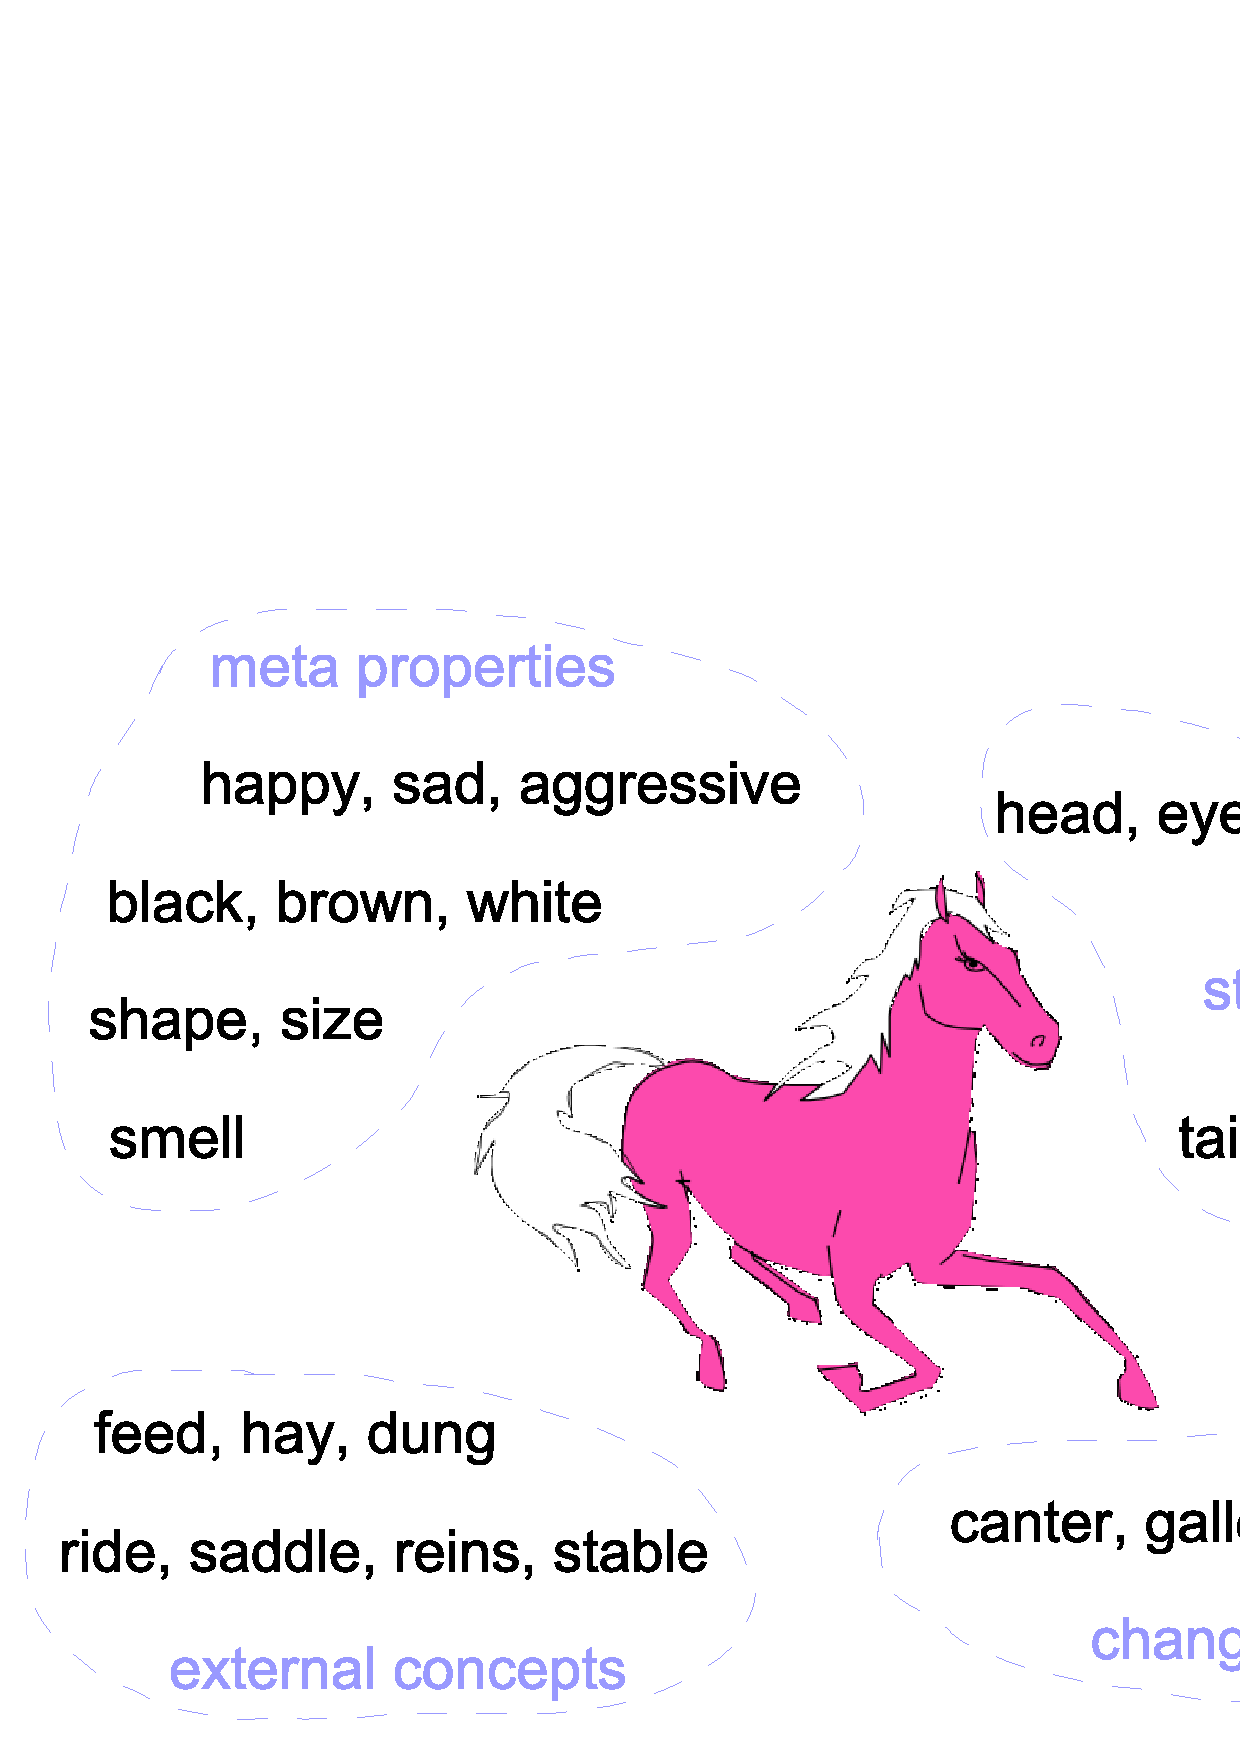
\includegraphics[scale=0.3,angle=-90]{graphic/horse.pdf}
        \caption{Concept of a Horse with Structure, Meta Properties and Logic}
        \label{horse_figure}
    \end{center}
\end{figure}

One might suggest to model properties like the position, size or colour of a
horse's leg as \emph{Part} of that leg. In fact, this is how classical
programming approaches its solutions.
\emph{Structured- and Procedural Programming} (SPP)
(section \ref{structured_and_procedural_programming_heading}), for example,
would probably use a structure called \emph{struct} or \emph{record}
representing the leg and a field standing for the leg's colour. Similarly,
\emph{Object Oriented Programming} (OOP)
(section \ref{object_oriented_programming_heading}) would use a class
representing the leg and an attribute standing for the leg's colour, which, in
Java source code, would look as follows:

\begin{scriptsize}
    \begin{verbatim}
    public class Leg {
        private String knee;
        private String hoof;
        private String colour;
    }
    \end{verbatim}
\end{scriptsize}

However, when following the modelling principles of human thinking (section
\ref{human_thinking_heading}), this is \emph{not} correct! It is true that in
everyday language, one tends to say \textit{A horse leg \emph{has a} colour.}
Unfortunately, this leads to the wrong assumption that a leg were made of a
colour. But this is not the case. A leg does not \emph{consist} of a colour in
the hierarchical meaning of a whole consisting of parts. The colour is rather
property information \emph{about} the leg. It seems there is no correct
expression in natural (English) language stating the property of something. The
\emph{IS-A} verbalisation is used to express that the leg belongs to a special
category of items, for example: \textit{A leg is a body element.} The
\emph{HAS-A} formulation is used to express that a leg as whole consists of
smaller parts, for example: \textit{A leg has a knee and it has a hoof.} But
which formulation expresses a property? Well, perhaps it would be best to say:
\textit{A leg IS-OF a colour.}

It seems that scientists (including the author of this work) and adults in
general have unlearnt to think simple like children. Scientists sometimes tend
to unnecessarily complicate things that can be described quite easy. Other
times, they simplify things which better be distinguished. And looking back
into the history of programming, one wonders who ever had this idea of mixing
structural elements, properties with meta information and logic algorithms into
just one structural entity as at least SPP (record, struct) and OOP (class) do.

The CYBOP knowledge schema introduced before takes care of these things and
distinguishes whole-part- from meta information. Actions (like the gallop of a
horse) causing some change in the model (horse) or its environment are called
\emph{Logic} in this work, since they follow certain rules. Chapter
\ref{state_and_logic_heading} will deal with these.
